\documentclass[12pt]{report}

\usepackage{forest}
\usepackage{caption}
\usepackage{booktabs}
\captionsetup[table]{skip=12pt}
\usepackage{xurl} % hỗ trợ ngắt URL rất tốt

\usepackage{hcmus-report-template}
\usepackage[shortlabels]{enumitem}
\usepackage{tocloft}
\usepackage{amsthm}
\theoremstyle{definition}
\newtheorem{problem}{Bài toán}[chapter]
\newtheorem{definition}{Định nghĩa}[chapter]

%--------------------------------------------------
% Paragraph layout
%--------------------------------------------------
\usepackage{indentfirst}
\setlength{\parindent}{3em}
\setlength{\parskip}{0pt}
\renewcommand{\baselinestretch}{1.5}

%--------------------------------------------------
% Sectioning
%--------------------------------------------------
\usepackage{titlesec}

% ===== CHAPTER FORMAT =====
\renewcommand{\thechapter}{\arabic{chapter}}

% Format heading chương: "Chương 1: Tổng quan nghiên cứu"
\titleformat{\chapter}[block]
  {\normalfont\huge\bfseries\centering}
  {Chương \thechapter.}{0.5em}{}

% ===== SECTION NUMBERING =====
\renewcommand{\thesection}{\thechapter.\arabic{section}}
\renewcommand{\thesubsection}{\thesection.\arabic{subsection}}
\renewcommand{\thesubsubsection}{\thesubsection.\arabic{subsubsection}}

% ===== SUBSUBSUBSECTION =====
\titleclass{\subsubsubsection}{straight}[\subsubsection]
\newcounter{subsubsubsection}[subsubsection]
\renewcommand{\thesubsubsubsection}{\thesubsubsection.\arabic{subsubsubsection}}

% ===== HEADING FORMAT =====
\titleformat{\section}{\normalfont\large\bfseries}{\thesection}{1em}{}
\titleformat{\subsection}{\normalfont\large\bfseries}{\thesubsection}{1em}{}
\titleformat{\subsubsection}{\normalfont\normalsize\bfseries}{\thesubsubsection}{1em}{}
\titleformat{\subsubsubsection}{\normalfont\normalsize\bfseries}{\thesubsubsubsection}{1em}{}

% ===== SPACING =====
\titlespacing*{\chapter}{0pt}{1em}{1em}
\titlespacing*{\section}{0em}{1em}{1em}
\titlespacing*{\subsection}{1em}{1em}{1em}
\titlespacing*{\subsubsection}{1em}{1em}{1em}
\titlespacing*{\subsubsubsection}{1em}{1em}{1em}

% ===== DEPTH =====
\setcounter{secnumdepth}{4}
\setcounter{tocdepth}{4}

% ===== RESET COUNTERS THEO CHAPTER =====
\makeatletter
\@addtoreset{section}{chapter}
\@addtoreset{subsection}{section}
\@addtoreset{subsubsection}{subsection}
\@addtoreset{subsubsubsection}{subsubsection}
\makeatother

%--------------------------------------------------
% TOC – subsubsubsection
%--------------------------------------------------
\makeatletter
\def\toclevel@subsubsubsection{4}
\newcommand{\l@subsubsubsection}{\@dottedtocline{4}{14em}{3em}}
\makeatother

%--------------------------------------------------
% TOC formatting với tocloft
%--------------------------------------------------

% 1. Dòng CHAPTER trong TOC: "Chương 1: Tổng quan nghiên cứu"
\renewcommand{\cftchapfont}{\bfseries}         % chữ đậm
\renewcommand{\cftchappagefont}{\bfseries}     % số trang đậm

% Thêm tiền tố & hậu tố quanh số chương
\renewcommand{\cftchappresnum}{Chương~}
\renewcommand{\cftchapaftersnum}{:\ }          % ra "Chương 1:"

% Độ rộng phần số chương trong TOC (tránh dính chữ)
\setlength{\cftchapnumwidth}{5.5em}              % tăng nếu vẫn bị dính

% Khoảng cách trước mỗi dòng chapter trong TOC
\setlength{\cftbeforechapskip}{0.75em}

% 2. Indent cho các level con trong TOC
\cftsetindents{chapter}{0em}{5.5em}
\cftsetindents{section}{2em}{3em}
\cftsetindents{subsection}{4em}{3.5em}
\cftsetindents{subsubsection}{6em}{4em}
% subsubsubsection được định nghĩa ở trên với indent 14em

% Độ rộng cột số trang
\cftsetpnumwidth{2.5em}

% hcmus-report-template đã load hyperref, nên chỉ cần hypersetup
\hypersetup{
  colorlinks=true,
  linkcolor=black,
}

%--------------------------------------------------
% Report info
%--------------------------------------------------

\newcommand{\coursename}{Khóa luận Tốt nghiệp Đại học}
\newcommand{\reporttitle}{BÁO CÁO KHÓA LUẬN TỐT NGHIỆP}
\newcommand{\reportname}{Phát triển mô hình hỏi đáp tin cậy bệnh lý về xương dựa trên mô hình ngôn ngữ lớn và truy xuất tăng cường sinh nội dung dựa trên văn bản}

\newcommand{\studentname}{Sinh viên thực hiện}
\newcommand{\teachername}{Giảng viên hướng dẫn}

% Header
\lhead{
  \coursename
}
\rhead{
}

% % Đảm bảo trang chapter có header (plain style mặc định không có header)
% \fancypagestyle{plain}{
%   \fancyhf{}
%   \lhead{\coursename}
%   \rhead{}
%   \fancyfoot[R]{Trang \thepage}
% }

% ============ DOCUMENT ============
\begin{document}


\begin{titlepage}
\newcommand{\HRule}{\rule{\linewidth}{0.5mm}}
\centering

\textsc{\LARGE TRƯỜNG ĐẠI HỌC KHOA HỌC TỰ NHIÊN}\\[0.2cm]
\textsc{\LARGE ĐẠI HỌC QUỐC GIA TP. HỒ CHÍ MINH}\\[0.3cm]
\textsc{\Large KHOA CÔNG NGHỆ THÔNG TIN}\\[0.5cm]


\includegraphics[scale=.30]{img/hcmus-logo.png}\\[0.8cm] 

\HRule \\[0.4cm]
{ 
\Large{\bfseries{\reporttitle}}\\[0.4cm]
\huge{\bfseries{\reportname}}
}\\[0.4cm]
\HRule \\[0.8cm]

\begin{minipage}[t]{0.45\textwidth}
\begin{flushleft} \large
\emph{Giảng viên hướng dẫn:} \\
\teachername
\end{flushleft}
\end{minipage}
~
\begin{minipage}[t]{0.45\textwidth}
\begin{flushright} \large
\emph{Sinh viên thực hiện:}\\
\studentname
\end{flushright}
\end{minipage}\\[1.5cm]

{\large Thành phố Hồ Chí Minh, \today}\\[1cm]

\vfill
\end{titlepage}

\pagenumbering{roman}

% \chapter*{Lời cảm ơn}
\addcontentsline{toc}{chapter}{Lời cảm ơn}

Nhóm xin trân trọng cảm ơn \textbf{PGS. TS. Lý Quốc Ngọc} đã trực tiếp hướng dẫn, giảng dạy các nội dung lý thuyết chính và định hướng khoa học cho đề tài.  
Nhóm cũng xin cảm ơn \textbf{ThS. Nguyễn Mạnh Hùng} và \textbf{ThS. Phạm Thanh Tùng} đã hỗ trợ trong quá trình thực hành và cung cấp các kiến thức thực nghiệm quan trọng, góp phần giúp nhóm hoàn thành báo cáo này.

\pagebreak

\tableofcontents
\clearpage
\listoffigures
\clearpage
\listoftables
\clearpage

\pagenumbering{arabic}
\setcounter{page}{1}

\chapter{Tổng quan nghiên cứu}

\section{Bối cảnh nghiên cứu}

\subsection{Thực trạng tiếp cận thông tin y khoa về bệnh lý về xương}
Trong bối cảnh y học hiện đại, khối lượng tri thức lâm sàng, các báo cáo thực nghiệm và phác đồ điều trị các bệnh lý về xương (bao gồm các bệnh lý phổ biến như loãng xương, thoái hóa xương khớp, gãy xương và viêm xương) đang gia tăng với tốc độ nhanh chóng \cite{who2022musculoskeletal}. Sự tích lũy tri thức y học quy mô lớn vừa mở ra cơ hội nâng cao chất lượng chăm sóc sức khỏe, vừa tạo ra thách thức lớn trong việc tiếp cận và khai thác thông tin chính xác \cite{medrag2024}. Thách thức này thể hiện rõ nét qua hai góc độ đối tượng sử dụng chính trong xã hội.


Đối với đội ngũ nhân viên y tế và sinh viên y khoa, việc tìm kiếm cũng như tổng hợp dữ liệu lâm sàng từ các bộ tài liệu y học chuyên ngành, sách giáo khoa hoặc cơ sở dữ liệu y sinh quy mô lớn đòi hỏi lượng thời gian đáng kể \cite{ortho_rag_13}. Trong môi trường thực hành áp lực cao, thời gian tra cứu kéo dài có thể làm chậm quá trình đưa ra quyết định chẩn đoán và chỉ định phác đồ điều trị \cite{medrag2024}. Vì vậy, việc ứng dụng các công cụ tự động hóa nhằm hỗ trợ tra cứu tri thức chuẩn xác với tốc độ phản hồi tức thì là yêu cầu vô cùng cấp thiết.

Đối với người bệnh và cộng đồng, xu hướng tự tra cứu triệu chứng và phương pháp điều trị các bệnh lý về xương trên mạng Internet ngày càng trở nên phổ biến. Tuy nhiên, nguồn tin trên không gian mạng thường rơi vào tình trạng nhiễu loạn và thiếu sự kiểm chứng từ chuyên gia. Việc tiếp cận các dữ liệu sai lệch dễ dẫn đến hành vi tự chẩn đoán sai, tự ý sử dụng thuốc không theo chỉ định, gây ra những biến chứng nguy hiểm. Thực trạng này đặt ra đòi hỏi phải xây dựng các giải pháp công nghệ có khả năng tư vấn y học chính xác, minh bạch, đảm bảo độ an toàn lâm sàng, khả năng đọc hiểu và sự đồng cảm với người bệnh \cite{ortho_rag_13}.

Song song với nhu cầu trên, các mô hình ngôn ngữ lớn (Large Language Model, LLM) đã đạt kết quả đáng chú ý trên nhiều bộ dữ liệu hỏi--đáp y khoa. Tuy nhiên, kết quả cao trên câu hỏi dạng thi hoặc trên một miền thử nghiệm hẹp chưa đồng nghĩa với khả năng sử dụng an toàn trong chăm sóc người bệnh. Khi câu hỏi dài, tình huống lâm sàng phức tạp hoặc thông tin bệnh nhân chưa đầy đủ, mô hình vẫn có thể tạo ra câu trả lời trôi chảy nhưng sai, thiếu cảnh báo hoặc không phù hợp với quy trình thực tế. Vì vậy, LLM trong nghiên cứu này được xem là công cụ hỗ trợ truy xuất và tổng hợp thông tin, không phải một hệ thống tự chủ thay thế bác sĩ.


\subsection{Sự tiến hóa của các hệ thống hỏi đáp y tế và điểm nghẽn công nghệ}
Để giải quyết bài toán tra cứu và tư vấn thông tin y tế, các hệ thống hỏi đáp tự động đã trải qua quá trình phát triển qua nhiều thế hệ công nghệ với những đặc trưng và giới hạn riêng biệt.

Thế hệ đầu tiên và thứ hai của các hệ thống hỏi đáp y tế được xây dựng dựa trên các hệ trợ giúp ra quyết định lâm sàng bằng tập luật \cite{rule_based_1, rule_based_2} kết hợp với thuật toán truy xuất từ khóa truyền thống như BM25 hay TF-IDF. Mặc dù các mô hình này đảm bảo tính an toàn cao nhờ tuân thủ nghiêm ngặt quy tắc logic định trước, chúng bộc lộ hạn chế lớn về tính linh hoạt. Do phụ thuộc vào việc khớp từ khóa chính xác, hệ thống không thể hiểu được ngữ nghĩa sâu xa, ngữ cảnh phức tạp hoặc các cách diễn đạt đa dạng trong câu hỏi ngôn ngữ tự nhiên từ người bệnh.

Sự xuất hiện của kiến trúc Transformer \cite{vaswani2017} đã đánh dấu bước chuyển mình sang thế hệ thứ ba với sự bùng nổ của các mô hình ngôn ngữ lớn (LLM). Nhờ được huấn luyện trên tập ngữ liệu khổng lồ, mô hình ngôn ngữ lớn sở hữu khả năng hiểu và sinh ngôn ngữ tự nhiên mượt mà, giải quyết rào cản giao tiếp giữa con người và máy tính. Tuy nhiên, khi áp dụng trực tiếp vào lĩnh vực y tế đòi hỏi sự chính xác tuyệt đối, mô hình ngôn ngữ lớn độc lập lại vấp phải rào cản chí mạng là hiện tượng ảo giác. Do bản chất của LLM là sinh văn bản bằng cách dự đoán xác suất từ ngữ tiếp theo hoàn toàn dựa vào tri thức tích lũy từ quá trình huấn luyện, mô hình có xu hướng tự tạo ra các thông tin sai lệch, sai liều lượng thuốc hoặc đưa ra phác đồ điều trị không có thực nhưng với văn phong hết sức tự tin. Trong ngành y tế, rủi ro ảo giác có thể gây ảnh hưởng trực tiếp đến an toàn tính mạng của người bệnh.

Ngoài hiện tượng ảo giác, LLM độc lập còn gặp ba giới hạn thực tế: tri thức trong tham số có thể trở nên lỗi thời khi hướng dẫn lâm sàng thay đổi; người dùng khó xác định nguồn bằng chứng hỗ trợ câu trả lời; và mô hình có thể khiến người dùng quá tin vào kết quả tự động. Các câu hỏi liên quan đến thuốc, chống chỉ định, chẩn đoán hoặc xử trí nguy cơ cao vì thế không nên được giải quyết chỉ bằng tri thức ghi nhớ sẵn của mô hình.




Để vượt qua điểm nghẽn ảo giác của các mô hình ngôn ngữ lớn độc lập, kiến trúc truy xuất tăng cường sinh nội dung (RAG) \cite{lewis2020, karpukhin2020} đã ra đời và tạo nên thế hệ thứ tư của các hệ thống hỏi đáp y tế.

\begin{definition}[Truy xuất Tăng cường Sinh nội dung (RAG)]
\label{def:rag}
Truy xuất Tăng cường Sinh nội dung (RAG) là một kỹ thuật AI và mẫu thiết kế hệ thống kết hợp mô hình ngôn ngữ lớn với hệ thống truy xuất thông tin bên ngoài như cơ sở tri thức, chỉ mục tìm kiếm hay cơ sở dữ liệu \cite{nist_ai_100_2e2025, cheng2025knowledge}, nhằm đảm bảo các phản hồi sinh ra được căn cứ trực tiếp trên dữ liệu miền chuyên biệt và có thể cập nhật theo thời gian thực. Hệ thống RAG thực hiện truy xuất nội dung liên quan dựa trên truy vấn người dùng \cite{nist_ai_100_2e2025} để cung cấp ngữ cảnh đầu vào \cite{gao2023}, cho phép mô hình sinh ra câu trả lời chính xác, có thể kiểm chứng mà không cần tái huấn luyện \cite{nist_ai_100_2e2025}.
\end{definition}


\noindent Định nghĩa trên được tổng hợp từ các góc nhìn bổ trợ lẫn nhau giữa tổ chức tiêu chuẩn (NIST \cite{nist_ai_100_2e2025}) và các nghiên cứu tổng quan học thuật tiêu biểu (Gao et al. \cite{gao2023}, Cheng et al. \cite{cheng2025knowledge}). Sự hội tụ giữa các định nghĩa này cho thấy RAG vừa là một mẫu thiết kế hệ thống giúp phản hồi luôn có căn cứ xác thực từ dữ liệu miền chuyên biệt, vừa là một kiến trúc linh hoạt cho phép cập nhật tri thức liên tục mà không cần tái huấn luyện mô hình \cite{nist_ai_100_2e2025, gao2023}. Đáng chú ý, RAG không bị giới hạn trong bất kỳ công nghệ truy xuất cụ thể nào mà có thể kết nối với đa dạng nguồn dữ liệu từ văn bản, cơ sở dữ liệu quan hệ đến đồ thị tri thức \cite{cheng2025knowledge}.


Chính nhờ cơ chế phân tách và xác thực tri thức chuẩn mực nêu trên, các nghiên cứu gần đây chứng minh rằng một mô hình mã nguồn mở quy mô vừa phải khi tích hợp RAG có thể đạt hiệu suất vượt trội hơn cả các mô hình độc quyền quy mô khổng lồ (như GPT-4) khi vận hành đơn lẻ không có cơ chế truy xuất \cite{medrag2024, gao2023}.

Tuy vậy, RAG không loại bỏ hoàn toàn hiện tượng ảo giác. Chất lượng câu trả lời vẫn phụ thuộc trực tiếp vào tài liệu được truy xuất: đoạn văn bản cũ, nhiễu, mâu thuẫn hoặc không đủ bằng chứng có thể khiến câu trả lời sai trở nên thuyết phục hơn vì có vẻ được hỗ trợ bởi nguồn tham khảo. Các kết quả trên MIRAGE cũng cho thấy hiệu quả thay đổi đáng kể theo kho tài liệu, bộ truy xuất và mô hình sinh được lựa chọn \cite{xiong2024mirage}. Trong hội thoại nhiều lượt, việc đưa toàn bộ lịch sử trao đổi vào câu lệnh còn có thể làm lệch ngữ cảnh. Do đó, lịch sử hội thoại phải được lọc, cô đọng và dùng để viết lại câu hỏi hiện tại thành một truy vấn độc lập trước khi truy xuất.

Một vấn đề khác là tính không đồng nhất của dữ liệu y khoa. Tài liệu có thể tồn tại dưới nhiều định dạng, chứa bảng hoặc sơ đồ khó trích xuất, sử dụng thuật ngữ khác nhau, có nhiều phiên bản, khác biệt giữa hướng dẫn quốc tế và quy trình địa phương, hoặc đã hết hiệu lực. Vì vậy, việc chỉ phân đoạn tài liệu và lưu vào cơ sở dữ liệu vector là chưa đủ; mỗi đoạn cần kèm siêu dữ liệu về nguồn, chuyên khoa, ngày ban hành, phiên bản, phạm vi áp dụng và trạng thái hiệu lực để phục vụ lọc, xếp hạng và trích dẫn. Thực trạng này dẫn đến nhu cầu về một quy trình tích hợp truy xuất lai, mô hình hỏi--đáp y khoa, lớp bảo đảm chất lượng và cơ chế lựa chọn giữa trả lời, từ chối trả lời hoặc chuyển đến chuyên gia.







\section{Động lực nghiên cứu}

Việc phát triển một giải pháp hỏi--đáp y khoa tin cậy mang ý nghĩa đối với cả nghiên cứu xử lý ngôn ngữ tự nhiên và hoạt động tra cứu thông tin sức khỏe.

\subsection{Ý nghĩa khoa học}

Về phương diện khoa học, đề tài thiết lập một khung thực nghiệm đầu cuối để khảo sát cách RAG vận hành trên ngữ liệu chuyên ngành về các bệnh lý về xương. Khung này cho phép so sánh RAG cơ sở với các cải tiến về truy xuất lai, tinh chỉnh mô hình bằng bằng chứng và kiểm soát phản hồi an toàn. Thay vì chỉ đo câu trả lời cuối cùng, việc đánh giá riêng ba tầng truy xuất, sinh nội dung và hỏi--đáp đầu cuối giúp xác định lỗi thuộc về kho tri thức, bộ truy xuất, mô hình sinh hay lớp bảo đảm chất lượng \cite{xiong2024mirage, medrag2024}.

Kết quả thực nghiệm có thể cung cấp mốc so sánh cho các nghiên cứu tiếp theo về hỏi--đáp y khoa tiếng Việt, đặc biệt trong việc cân bằng giữa khả năng trả lời, độ bám sát nguồn và hành vi từ chối hợp lý.

\subsection{Ý nghĩa thực tiễn}

Về phương diện ứng dụng, hệ thống hướng đến việc rút ngắn thời gian tra cứu tài liệu chuyên khoa cho nhân viên y tế và sinh viên, đồng thời cung cấp cho người bệnh một kênh tham khảo ban đầu có nguồn bằng chứng rõ ràng \cite{ortho_rag_13}. Cơ chế Answer--Abstain--Escalate giúp biểu đạt giới hạn của hệ thống: chỉ trả lời khi đủ căn cứ, từ chối khi chưa chắc chắn và khuyến nghị gặp chuyên gia khi có nguy cơ.

Giá trị thực tiễn của giải pháp còn nằm ở khả năng cập nhật kho tri thức mà không phải huấn luyện lại toàn bộ LLM, cũng như việc đặt bảo vệ dữ liệu cá nhân và giám sát của con người thành điều kiện vận hành. Hệ thống vì thế đóng vai trò hỗ trợ tra cứu và giáo dục sức khỏe, không thay thế quyết định lâm sàng của bác sĩ.

% Nội dung thách thức và khoảng trống nghiên cứu đã được hợp nhất vào phần thực trạng.
\section{Phát biểu bài toán và hai pipeline của hệ thống}

\subsection{Đầu vào và đầu ra của bài toán}

Nghiên cứu xem xét bài toán hỏi--đáp y khoa tin cậy dựa trên kiến trúc truy xuất tăng cường sinh nội dung (Retrieval-Augmented Generation, RAG) \cite{lewis2020}. Hệ thống kết hợp tri thức y khoa đã được kiểm chứng với mô hình ngôn ngữ lớn (Large Language Model, LLM), qua đó ưu tiên bằng chứng truy xuất thay vì chỉ dựa vào tri thức được ghi nhớ trong tham số mô hình.

Trong giai đoạn huấn luyện, đầu vào thứ nhất là tập tài liệu y khoa đã được kiểm chứng
\[
    D = \{d_1,d_2,\ldots,d_{N_D}\},
\]
trong đó $d_j$ là tài liệu thứ $j$ và $N_D$ là số tài liệu. Tập $D$ có thể bao gồm giáo trình, hướng dẫn lâm sàng, phác đồ chẩn đoán--điều trị và các cặp hỏi--đáp đã được chuyên gia xác nhận. Đầu vào thứ hai là bộ dữ liệu hỏi--đáp
\[
    \mathcal{T}_{\mathrm{QA}}
    = \{(q_i,u_i,h_i,y_i^*)\}_{i=1}^{N_Q},
\]
trong đó $N_Q$ là số mẫu huấn luyện; $q_i$ là câu hỏi y khoa; $u_i$ là phần bối cảnh bệnh nhân được phép sử dụng; $h_i$ là lịch sử hội thoại; và $y_i^*$ là câu trả lời chuẩn của mẫu thứ $i$.

Sau tiền xử lý, tập tài liệu $D$ được phân chia thành tập các đoạn văn bản
\[
    C = \{c_1,c_2,\ldots,c_{N_C}\},
\]
trong đó $c_j$ là một đoạn văn bản (chunk) và $N_C$ là tổng số đoạn. Các đoạn cùng siêu dữ liệu và biểu diễn tìm kiếm được lưu trong chỉ mục tri thức $I$. Với mỗi mẫu hỏi--đáp, hệ thống truy xuất tập bằng chứng $C_i^* \subseteq C$ để hình thành mẫu tinh chỉnh $(q_i,u_i,h_i,C_i^*,y_i^*)$.

Trong giai đoạn suy diễn, đầu vào của một lượt hỏi được biểu diễn bởi
\[
    X=(q,u,h,I),
\]
trong đó $q$ là câu hỏi hiện tại, $u$ là bối cảnh bệnh nhân cần thiết và được phép sử dụng, $h$ là lịch sử hội thoại, còn $I$ là chỉ mục tri thức đã được xây dựng từ tập tài liệu $D$.

Đầu ra chính không chỉ là một câu trả lời mà là cặp
\[
    O=(\hat{y},d),
    \qquad
    d\in\Delta=\{\text{Answer},\text{Abstain},\text{Escalate}\},
\]
trong đó $\hat{y}$ là phản hồi cuối cùng và $d$ là quyết định thuộc tập hành động $\Delta$. Quyết định \emph{Answer} được chọn khi bằng chứng đủ mạnh và câu trả lời an toàn; \emph{Abstain} biểu thị việc từ chối trả lời khi bằng chứng thiếu, mâu thuẫn hoặc độ tin cậy thấp; còn \emph{Escalate} chuyển người dùng đến bác sĩ hoặc chuyên gia khi tình huống có nguy cơ cao, khẩn cấp hay vượt phạm vi của hệ thống. Khi phù hợp, đầu ra còn kèm các đoạn bằng chứng, nguồn trích dẫn, độ tin cậy và cảnh báo an toàn.

\subsection{Các tham số cần học và biến trung gian}

Các ẩn cần tìm của bài toán được chia thành hai nhóm. Nhóm thứ nhất là bộ tham số được học hoặc hiệu chỉnh trong giai đoạn huấn luyện:
\[
    \Theta=\{\phi,\theta,\psi\},
\]
trong đó $\phi$ là tham số của bộ truy xuất, quyết định cách biểu diễn và chấm điểm độ liên quan giữa truy vấn với đoạn tài liệu; $\theta$ là tham số của LLM dùng để sinh câu trả lời; và $\psi$ là tham số cùng các ngưỡng của lớp bảo đảm chất lượng, dùng để đánh giá bằng chứng, độ an toàn và lựa chọn quyết định cuối cùng.

Nhóm thứ hai gồm các biến phải suy ra cho mỗi lượt hỏi:
\begin{itemize}
    \item $q'$: truy vấn độc lập đã được chuẩn hóa từ câu hỏi hiện tại và ngữ cảnh liên quan;
    \item $m$ và $e$: lần lượt là ý định y khoa và tập thực thể y khoa được nhận diện trong truy vấn;
    \item $\mathbf{z}_q\in\mathbb{R}^{d_e}$: vector nhúng $d_e$ chiều của truy vấn;
    \item $C^*=\{c_{(1)},\ldots,c_{(k)}\}\subseteq C$: tập $k$ đoạn bằng chứng liên quan nhất;
    \item $\widetilde{y}$: câu trả lời nháp do LLM sinh ra;
    \item $\mathbf{v}$: vector điểm chất lượng gồm độ liên quan, độ bám sát bằng chứng, tính đầy đủ, độ chính xác trích dẫn, độ an toàn và độ tin cậy;
    \item $d\in\Delta$: quyết định cuối cùng của hệ thống.
\end{itemize}

\subsection{Nguyên lý và phát biểu toán học tổng quát}

Nguyên lý cốt lõi của bài toán là sinh phản hồi có căn cứ và có chọn lọc. Bộ truy xuất cung cấp bằng chứng từ kho tri thức đã kiểm chứng; LLM tổng hợp câu trả lời trên bằng chứng đó; lớp bảo đảm chất lượng có quyền ngăn câu trả lời hoặc chuyển đến chuyên gia khi điều kiện an toàn không được đáp ứng. Toàn bộ bài toán được biểu diễn bởi ánh xạ
\[
    F_{\phi,\theta,\psi}:(q,u,h,I)\longrightarrow(C^*,\hat{y},d).
\]
Trong đó, các thành phần đầu vào, đầu ra và tham số đã được định nghĩa ở hai mục trên. Gọi $\mathcal{T}$ là phân phối dữ liệu đánh giá và $\mathcal{U}$ là hàm hữu dụng y khoa phản ánh đồng thời độ chính xác, độ bám sát bằng chứng, độ an toàn và chất lượng quyết định. Bài toán tối ưu tổng quát là
\[
    (\phi^*,\theta^*,\psi^*)
    =\arg\max_{\phi,\theta,\psi}
    \mathbb{E}_{X\sim\mathcal{T}}
    \left[\mathcal{U}\bigl(F_{\phi,\theta,\psi}(X)\bigr)\right].
\]
Việc tối ưu phải thỏa mãn các ràng buộc về thời gian phản hồi, bộ nhớ và độ dài cửa sổ ngữ cảnh. Các phép biến đổi cụ thể tạo nên ánh xạ $F_{\phi,\theta,\psi}$ được trình bày trong hai pipeline dưới đây.

\subsection{Pipeline huấn luyện}

Pipeline huấn luyện tạo kho tri thức có thể truy xuất, dữ liệu tinh chỉnh RAG, LLM chuyên biệt và các ngưỡng chất lượng--an toàn. Tổng quan pipeline được trình bày trong Hình~\ref{fig:training-pipeline}; quy trình gồm năm bước sau.

\begin{figure}[htbp]
    \centering
    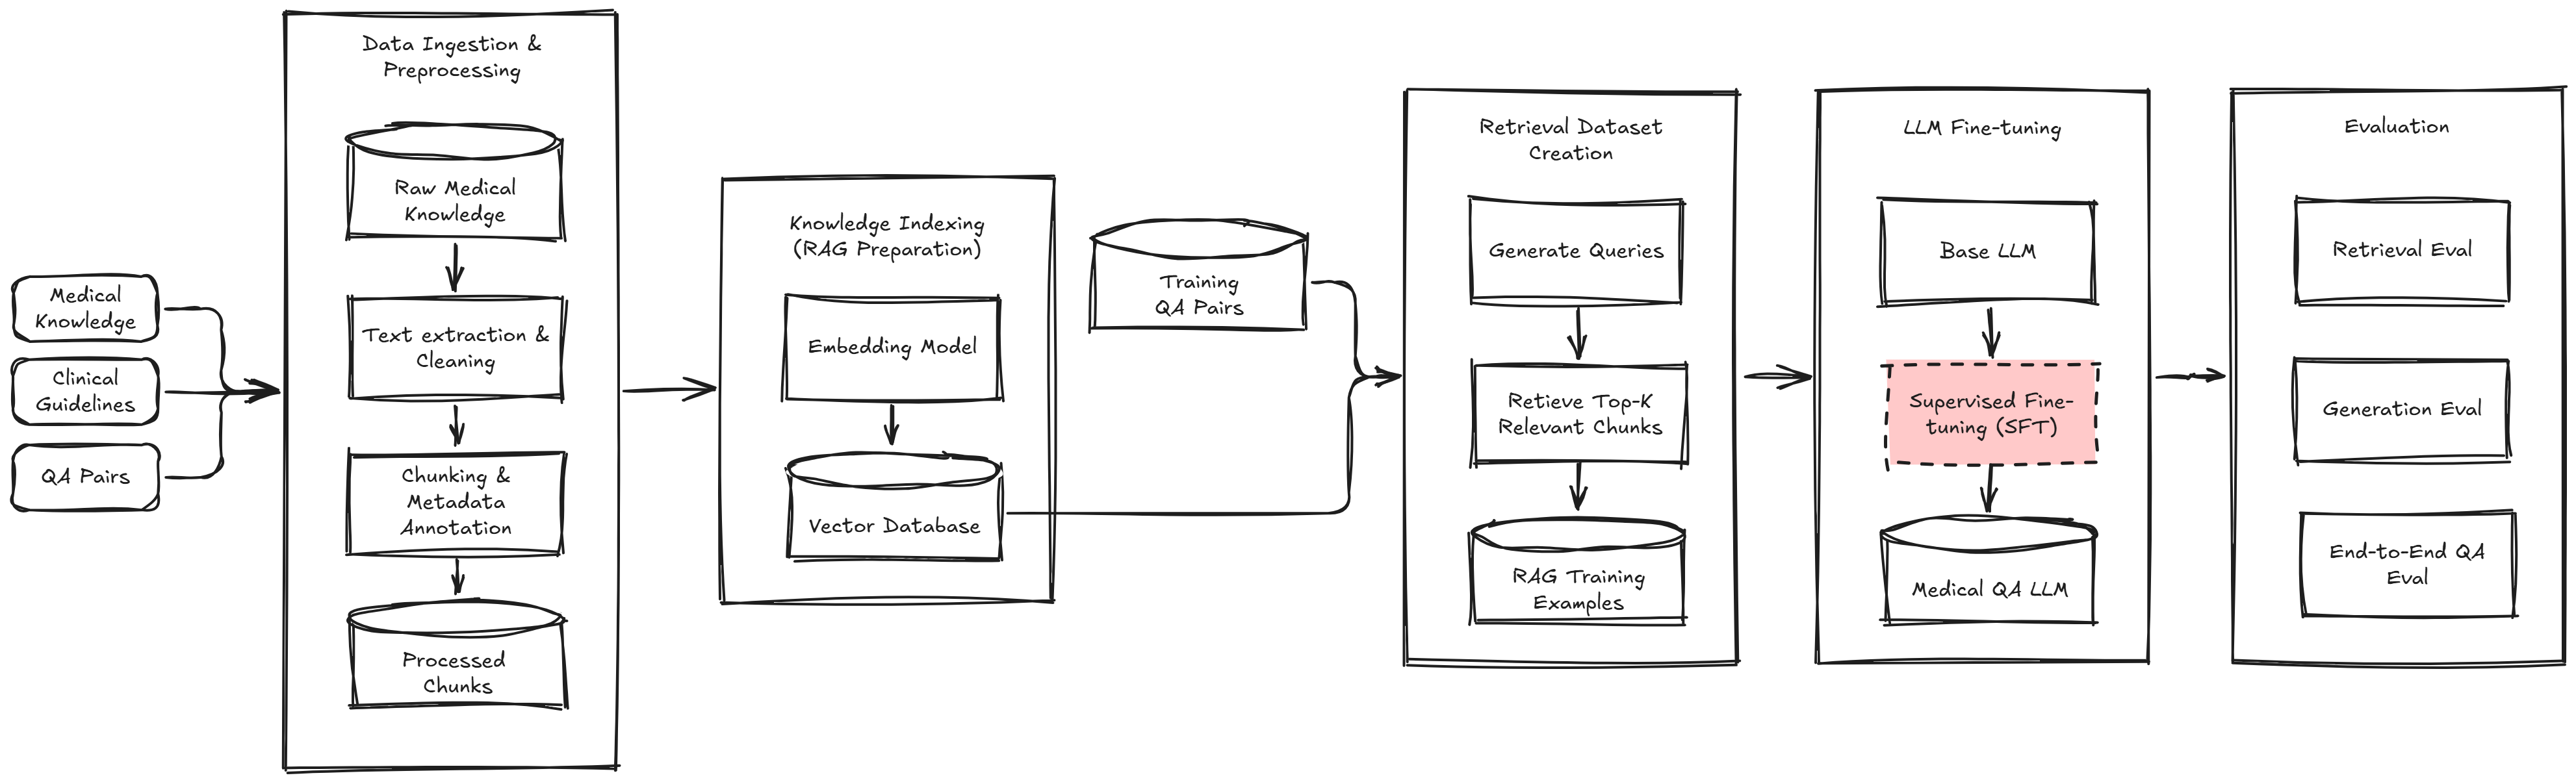
\includegraphics[width=\textwidth]{img/training_pipeline.png}
    \caption{Pipeline huấn luyện của hệ thống hỏi--đáp y khoa dựa trên RAG}
    \label{fig:training-pipeline}
\end{figure}

\subsubsection{Bước 1: Thu thập và tiền xử lý dữ liệu}

Tập tài liệu $D$ được thu thập từ các nguồn y khoa chính thống như giáo trình, hướng dẫn lâm sàng, phác đồ chẩn đoán--điều trị và các cặp hỏi--đáp đã được kiểm chứng. Tài liệu thô ở dạng PDF, Word, HTML hoặc cơ sở dữ liệu được trích xuất văn bản; loại bỏ đầu trang, chân trang, ký tự lỗi và nội dung trùng lặp; chuẩn hóa thuật ngữ, đơn vị và định dạng; đồng thời loại bỏ hoặc ẩn thông tin nhận dạng bệnh nhân.

Hàm phân đoạn $f_{\mathrm{chunk}}$ chuyển tập tài liệu thành các đoạn:
\[
    C=f_{\mathrm{chunk}}(D;\ell,s),
\]
trong đó $\ell$ là kích thước đoạn và $s$ là bước trượt. Mỗi đoạn $c_j$ được gắn siêu dữ liệu $\mu_j$ gồm tên tài liệu, chuyên khoa, chủ đề, tổ chức phát hành, ngày ban hành, phiên bản, vị trí trong tài liệu, phạm vi áp dụng, trạng thái hiệu lực và độ tin cậy của nguồn. Đầu ra của bước này là tập các đoạn sạch $(c_j,\mu_j)$ đủ thông tin để truy xuất và trích dẫn.

\subsubsection{Bước 2: Lập chỉ mục tri thức và huấn luyện bộ truy xuất}

Mô hình nhúng $E_{\phi}$ biến mỗi đoạn $c_j$ thành vector $\mathbf{z}_j=E_{\phi}(c_j)\in\mathbb{R}^{d_e}$. Vector, nội dung đoạn, siêu dữ liệu và thông tin trích dẫn được lưu trong chỉ mục đặc $I_{\mathrm{dense}}$; đồng thời, biểu diễn từ khóa được lưu trong chỉ mục thưa $I_{\mathrm{sparse}}$. Chỉ mục tri thức hoàn chỉnh là $I=(I_{\mathrm{dense}},I_{\mathrm{sparse}})$.

Điểm truy xuất lai giữa truy vấn $q$ và đoạn $c$ được xác định bởi
\[
    s_{\phi}(q,c)
    =\alpha s_{\mathrm{dense},\phi}(q,c)
    +(1-\alpha)s_{\mathrm{sparse}}(q,c),
\]
trong đó $s_{\mathrm{dense},\phi}$ là điểm tương đồng ngữ nghĩa, $s_{\mathrm{sparse}}$ là điểm khớp từ khóa và $\alpha\in[0,1]$ là hệ số phối hợp hai thành phần.

Khi có nhãn đoạn dương và đoạn âm, bộ truy xuất được huấn luyện để đưa câu hỏi gần đoạn liên quan và xa các đoạn không liên quan. Với $c_i^+$ là đoạn đúng và $\mathcal{B}_i^-$ là tập đoạn âm hoặc âm khó của câu hỏi $q_i$, hàm mất mát truy xuất được xác định bởi \cite{karpukhin2020}
\[
    \mathcal{L}_{\mathrm{ret}}(\phi)
    =-\sum_i\log
    \frac{\exp(s_{\phi}(q_i,c_i^+))}
    {\exp(s_{\phi}(q_i,c_i^+))+
     \sum_{c^-\in\mathcal{B}_i^-}\exp(s_{\phi}(q_i,c^-))}.
\]
Nếu tham số $\phi$ được cập nhật, toàn bộ vector đoạn phải được tạo lại và chỉ mục $I_{\mathrm{dense}}$ phải được cập nhật trước các bước tiếp theo.

\subsubsection{Bước 3: Tạo dữ liệu huấn luyện RAG}

Từ bộ $\mathcal{T}_{\mathrm{QA}}$, câu hỏi được chuẩn hóa hoặc mở rộng bằng các cách diễn đạt tương đương, câu hỏi sinh từ tài liệu, câu hỏi nối tiếp trong hội thoại và trường hợp cố ý thiếu bằng chứng. Với mỗi câu hỏi, hệ thống thực hiện truy xuất lai, lấy Top-$k$ đoạn, lọc theo siêu dữ liệu và có thể xếp hạng lại để thu được $C_i^*$.

Tập mẫu tinh chỉnh được tạo thành
\[
    \mathcal{T}_{\mathrm{RAG}}
    =\{(q_i,u_i,\bar{h}_i,C_i^*,y_i^*,d_i^*)\}_{i=1}^{N_Q},
\]
trong đó $\bar{h}_i$ là lịch sử đã cô đọng và $d_i^*\in\Delta$ là nhãn hành động chuẩn. Mỗi mẫu dạy mô hình đọc bằng chứng, trả lời dựa trên nguồn, trích dẫn đúng, biểu đạt độ không chắc chắn, từ chối khi bằng chứng không đủ và chuyển chuyên gia đối với tình huống nguy cơ cao.

\subsubsection{Bước 4: Tinh chỉnh LLM và lớp quyết định}

LLM nền được tinh chỉnh có giám sát (Supervised Fine-Tuning, SFT) trên $\mathcal{T}_{\mathrm{RAG}}$. Hàm mất mát sinh câu trả lời là
\[
    \mathcal{L}_{\mathrm{gen}}(\theta)
    =-\sum_i\sum_{t=1}^{T_i}
    \log P_{\theta}\!\left(
        y_{i,t}^*\mid y_{i,<t}^*,q_i,u_i,\bar{h}_i,C_i^*
    \right),
\]
trong đó $T_i$ là độ dài câu trả lời chuẩn và $y_{i,<t}^*$ là các token đứng trước vị trí $t$. Lớp bảo đảm chất lượng được học hoặc hiệu chỉnh bằng hàm mất mát $\mathcal{L}_{\mathrm{safe}}(\psi)$, bao gồm lỗi phân loại quyết định $d_i^*$ và các lỗi liên quan đến độ bám sát bằng chứng, trích dẫn và an toàn.

Hàm mục tiêu tổng hợp được viết dưới dạng
\[
    \mathcal{L}
    =\lambda_{\mathrm{ret}}\mathcal{L}_{\mathrm{ret}}
    +\lambda_{\mathrm{gen}}\mathcal{L}_{\mathrm{gen}}
    +\lambda_{\mathrm{safe}}\mathcal{L}_{\mathrm{safe}},
\]
trong đó các hệ số không âm $\lambda_{\mathrm{ret}}$, $\lambda_{\mathrm{gen}}$ và $\lambda_{\mathrm{safe}}$ kiểm soát đóng góp tương đối của ba mục tiêu. Các thành phần có thể được tối ưu theo từng giai đoạn, nhưng phải được đánh giá lại trong cùng một pipeline đầu cuối.

\subsubsection{Bước 5: Đánh giá và lựa chọn mô hình}

Đánh giá được thực hiện ở ba tầng:
\begin{itemize}
    \item \textbf{Tầng truy xuất:} sử dụng $\mathrm{Recall}@k$, $\mathrm{Precision}@k$, Mean Reciprocal Rank (MRR), normalized Discounted Cumulative Gain (nDCG) và tỷ lệ tài liệu chuẩn xuất hiện trong Top-$k$ để kiểm tra khả năng tìm đúng bằng chứng \cite{xiong2024mirage}.
    \item \textbf{Tầng sinh câu trả lời:} đánh giá độ chính xác y khoa, độ liên quan, độ trung thực và bám sát bằng chứng, tính đầy đủ, tỷ lệ ảo giác, độ chính xác của trích dẫn và độ an toàn \cite{ragas2023, medtrustrag}.
    \item \textbf{Tầng hỏi--đáp đầu cuối:} đánh giá toàn bộ chuỗi từ câu hỏi, truy xuất, xây dựng câu lệnh, sinh câu trả lời, kiểm tra chất lượng đến quyết định cuối cùng; trong đó kiểm tra riêng khả năng trả lời đúng, từ chối đúng và chuyển chuyên gia đúng.
\end{itemize}

Đầu ra của pipeline huấn luyện gồm chỉ mục tri thức $I$, tập mẫu $\mathcal{T}_{\mathrm{RAG}}$, LLM hỏi--đáp y khoa đã tinh chỉnh, tham số hoặc ngưỡng chất lượng--an toàn $\psi$, kết quả đánh giá và checkpoint mô hình tốt nhất.

\subsection{Pipeline suy diễn}

Pipeline suy diễn sử dụng các thành phần đã tạo trong huấn luyện để xử lý một lượt hỏi qua năm bước. Luồng xử lý từ đầu vào đến quyết định Answer--Abstain--Escalate được minh họa trong Hình~\ref{fig:inference-pipeline}.

\begin{figure}[htbp]
    \centering
    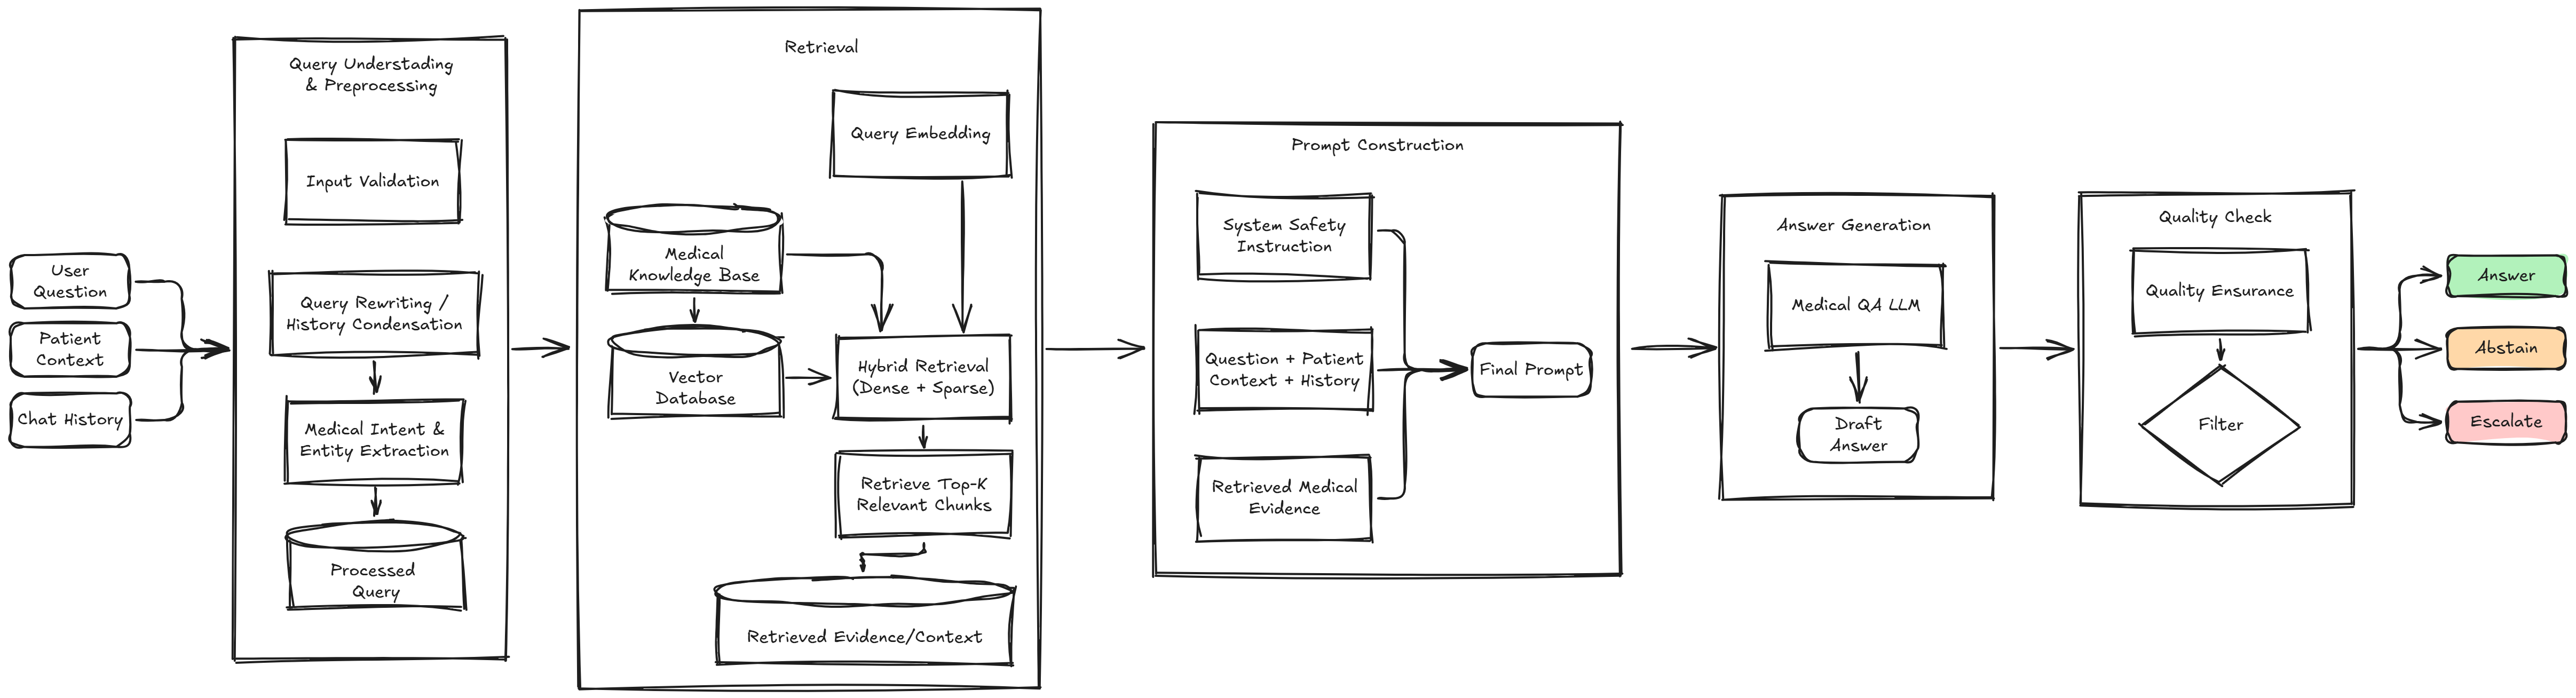
\includegraphics[width=\textwidth]{img/infer_pipeline.png}
    \caption{Pipeline suy diễn và cơ chế quyết định phản hồi của hệ thống}
    \label{fig:inference-pipeline}
\end{figure}

\subsubsection{Bước 1: Hiểu và tiền xử lý truy vấn}

Hệ thống tiếp nhận câu hỏi $q$, bối cảnh bệnh nhân $u$ và lịch sử hội thoại $h$. Bối cảnh bệnh nhân có thể gồm tuổi, giới tính, triệu chứng, tiền sử, thuốc đang dùng, dị ứng hoặc kết quả xét nghiệm, nhưng chỉ phần dữ liệu cần thiết và được phép mới được sử dụng. Đầu vào được kiểm tra về định dạng, phạm vi, dữ liệu nhạy cảm và dấu hiệu cấp cứu.

Lịch sử $h$ được lọc và cô đọng thành $\bar{h}$ thay vì đưa nguyên văn toàn bộ hội thoại vào câu lệnh. Hàm $f_{\mathrm{pre}}$ viết lại câu hỏi nối tiếp thành truy vấn độc lập $q'$, nhận diện ngôn ngữ, chuẩn hóa thuật ngữ Việt--Anh, xác định ý định $m$ và trích xuất các thực thể $e$ như bệnh, thuốc, triệu chứng, liều lượng, thời gian và yếu tố nguy cơ.

\subsubsection{Bước 2: Truy xuất bằng chứng}

Truy vấn $q'$ được mã hóa thành $\mathbf{z}_q$ bằng cùng mô hình $E_{\phi}$ đã dùng khi lập chỉ mục. Hệ thống kết hợp truy xuất đặc và truy xuất thưa theo điểm $s_{\phi}$, lấy Top-$k$ đoạn rồi lọc theo chuyên khoa, ngày ban hành, trạng thái hiệu lực và phạm vi áp dụng. Một bộ xếp hạng lại có thể đưa bằng chứng phù hợp nhất lên đầu và loại các đoạn nhiễu hoặc trùng lặp.

Đầu ra là tập $C^*$, trong đó mỗi đoạn đi kèm nội dung, nguồn tài liệu, ngày hoặc phiên bản, điểm liên quan và siêu dữ liệu cần thiết để trích dẫn. Nếu bằng chứng không đủ hoặc các nguồn mâu thuẫn nghiêm trọng, tín hiệu này được chuyển đến lớp quyết định thay vì bị che giấu ở bước sinh.

\subsubsection{Bước 3: Xây dựng câu lệnh}

Câu lệnh $P$ gồm chỉ dẫn an toàn $I_{\mathrm{safe}}$, truy vấn đã xử lý $q'$, phần bối cảnh bệnh nhân $u$ có liên quan, lịch sử cô đọng $\bar{h}$, tập bằng chứng $C^*$ và định dạng đầu ra yêu cầu. Chỉ dẫn an toàn buộc mô hình ưu tiên bằng chứng, không tự tạo chẩn đoán chắc chắn hoặc liều thuốc khi thiếu dữ liệu, nêu rõ giới hạn, và đề nghị gặp chuyên gia khi có dấu hiệu nguy hiểm. Mỗi đoạn bằng chứng được đánh dấu nguồn rõ ràng để hỗ trợ kiểm tra trích dẫn.

\subsubsection{Bước 4: Sinh câu trả lời nháp}

LLM hỏi--đáp y khoa với tham số $\theta^*$ đọc câu lệnh $P$ và tạo câu trả lời nháp $\widetilde{y}$. Câu trả lời có thể gồm nội dung chính, giải thích, bằng chứng hỗ trợ, trích dẫn, cảnh báo và mức độ không chắc chắn. Bản nháp chưa được gửi trực tiếp cho người dùng mà phải qua lớp bảo đảm chất lượng.

\subsubsection{Bước 5: Kiểm tra chất lượng và ra quyết định}

Lớp $g_{\psi^*}$ đánh giá bản nháp theo các tiêu chí: trả lời đúng trọng tâm; được bằng chứng hỗ trợ; không thêm luận điểm ngoài nguồn; trích dẫn đúng; không bỏ sót cảnh báo quan trọng; không gây hại; nhất quán với bối cảnh bệnh nhân; và đủ tin cậy để phản hồi. Kết quả tạo quyết định cuối cùng:
\begin{itemize}
    \item \textbf{Answer:} bằng chứng đủ mạnh, câu trả lời bám sát tài liệu, trích dẫn hợp lệ và không phát hiện rủi ro nghiêm trọng;
    \item \textbf{Abstain:} không tìm được bằng chứng phù hợp, nguồn mâu thuẫn, câu hỏi thiếu thông tin, độ tin cậy thấp hoặc nằm ngoài phạm vi hệ thống;
    \item \textbf{Escalate:} có dấu hiệu cấp cứu, cần khám trực tiếp, liên quan đến quyết định điều trị nguy cơ cao, phản ứng thuốc nghiêm trọng hoặc cần bác sĩ đánh giá hồ sơ đầy đủ.
\end{itemize}

Như vậy, hai pipeline liên kết với nhau qua chỉ mục tri thức $I$, mô hình truy xuất $\phi^*$, LLM $\theta^*$ và lớp quyết định $\psi^*$. Sự liên kết này bảo đảm các ký hiệu và thành phần được sử dụng thống nhất từ xây dựng dữ liệu, huấn luyện đến vận hành thực tế.

\section{Đóng góp của nghiên cứu}

Nghiên cứu mang lại ba đóng góp cốt lõi cả về phương pháp luận khoa học và giá trị ứng dụng thực tiễn:

\begin{enumerate}[label=(\arabic*)]
    \item \textbf{Chuẩn hóa khung hệ thống RAG cho bài toán hỏi đáp y khoa:} Đề xuất, cài đặt và đánh giá toàn diện một quy trình RAG tiêu chuẩn kết hợp giữa mô hình nhúng văn bản và mô hình ngôn ngữ lớn, được tối ưu hóa cho dữ liệu chuyên sâu về các bệnh lý về xương. Quy trình này thiết lập mốc so sánh (baseline) được thực nghiệm bài bản, tạo nền tảng khoa học cho việc đánh giá các kỹ thuật RAG nâng cao trong tương lai.
    
    \item \textbf{Xây dựng bộ dữ liệu và bộ câu hỏi đánh giá chuyên ngành về các bệnh lý về xương:} Thu thập, tiền xử lý và chuẩn hóa bộ ngữ liệu y khoa chuyên sâu từ các nguồn tài liệu chính thống, đồng thời xây dựng tập câu hỏi thực nghiệm nhằm cung cấp tài nguyên dữ liệu phục vụ nghiên cứu hỏi đáp y tế.
    
    \item \textbf{Thực nghiệm và đánh giá hệ thống:} Thực hiện đánh giá thực nghiệm toàn diện trên kiến trúc RAG đề xuất nhằm đo lường khả năng giảm thiểu hiện tượng ảo giác, nâng cao độ trung thực và độ tin cậy của câu trả lời trong tư vấn thông tin y học.
\end{enumerate}




% References
\cleardoublepage
\phantomsection
\addcontentsline{toc}{section}{Tài liệu tham khảo}

\begin{thebibliography}{99}

\bibitem{rule_based_1}
L. L. E., et al. (2018).
\href{https://doi.org/10.1016/j.ijmedinf.2018.01.018}{A rule-based clinical decision model to support interpretation of multiple data in health examinations}.
\textit{International Journal of Medical Informatics}, 112, 128--135. \url{https://doi.org/10.1016/j.ijmedinf.2018.01.018}.

\bibitem{rule_based_2}
K. M., et al. (2021).
\href{https://doi.org/10.1109/ACCESS.2021.3066311}{A Hybrid AI and Rule-Based Decision Support System for Disease Diagnosis and Management Using Labs}.
\textit{IEEE Access}, 9, 45120--45132. \url{https://doi.org/10.1109/ACCESS.2021.3066311}.

\bibitem{vaswani2017}
Vaswani, A., Shazeer, N., Parmar, N., Uszkoreit, J., Jones, L., Gomez, A. N., Kaiser, Ł., \& Polosukhin, I. (2017).
\href{https://arxiv.org/abs/1706.03762}{Attention is all you need}.
In \textit{Advances in Neural Information Processing Systems} (Vol. 30, pp. 5998--6008). \url{https://arxiv.org/abs/1706.03762}.

\bibitem{karpukhin2020}
Karpukhin, V., Oğuz, B., Min, S., Lewis, P., Wu, L., Edunov, S., Chen, D., \& Yih, W. T. (2020).
\href{https://arxiv.org/abs/2004.04906}{Dense passage retrieval for open-domain question answering}.
\textit{arXiv preprint arXiv:2004.04906}. \url{https://arxiv.org/abs/2004.04906}.

\bibitem{lewis2020}
Lewis, P., Perez, E., Piktus, A., Petroni, F., Karpukhin, V., Goyal, N., Küttler, H., Lewis, M., Yih, W. T., Rocktäschel, T., Riedel, S., \& Kiela, D. (2020).
\href{https://arxiv.org/abs/2005.11401}{Retrieval-augmented generation for knowledge-intensive NLP tasks}.
In \textit{Advances in Neural Information Processing Systems} (Vol. 33, pp. 9459--9474). \url{https://arxiv.org/abs/2005.11401}.

\bibitem{gao2023}
Gao, Y., Xiong, Y., Gao, X., Jia, K., Pan, J., Bi, Y., Dai, Y., Sun, J., \& Wang, H. (2023).
\href{https://arxiv.org/abs/2312.10997}{Retrieval-augmented generation for large language models: A survey}.
\textit{arXiv preprint arXiv:2312.10997}. \url{https://arxiv.org/abs/2312.10997}.

\bibitem{ragas2023}
Es, S., James, J., Espinosa-Anke, L., \& Schockaert, S. (2023).
\href{https://arxiv.org/abs/2309.15217}{RAGAS: Automated Evaluation of Retrieval Augmented Generation}.
\textit{arXiv preprint arXiv:2309.15217}. \url{https://arxiv.org/abs/2309.15217}.


\bibitem{xiong2024mirage}
Xiong, G., Jin, Q., Lu, Z., \& Zhang, A. (2024).
\href{https://arxiv.org/abs/2411.09213}{Benchmarking Retrieval-Augmented Generation for Medicine}.
In \textit{Findings of the Association for Computational Linguistics (ACL)}. \textit{arXiv preprint arXiv:2411.09213}. \url{https://arxiv.org/abs/2411.09213}.

\bibitem{medrag2024}
Xiong, G., et al. (2024).
\href{https://arxiv.org/abs/2404.14746}{MedRAG: Towards Reliable Medical Question Answering with Retrieval-Augmented Generation}.
\textit{arXiv preprint arXiv:2404.14746}. \url{https://arxiv.org/abs/2404.14746}.

\bibitem{imedrag}
Kim, J., et al. (2024).
\href{https://arxiv.org/abs/2405.03124}{Improving Retrieval-Augmented Generation in Medicine with Iterative Follow-up Questions}.
\textit{arXiv preprint arXiv:2405.03124}. \url{https://arxiv.org/abs/2405.03124}.

\bibitem{medtrustrag}
Zhang, H., et al. (2024).
\href{https://arxiv.org/abs/2406.08210}{MedTrust-RAG: Evidence Verification and Trust Alignment for Biomedical Question Answering}.
\textit{arXiv preprint arXiv:2406.08210}. \url{https://arxiv.org/abs/2406.08210}.


\bibitem{ortho_rag_13}
Mueller, M., et al. (2024).
\href{https://doi.org/10.2196/54321}{Development and Evaluation of a Retrieval-augmented Generation Chatbot for Orthopedic and Trauma Surgery Patient Education: A Mixed-methods Study}.
\textit{JMIR AI}, 3, e54321. \url{https://doi.org/10.2196/54321}.

\bibitem{nist_ai_100_2e2025}
National Institute of Standards and Technology. (2025).
\href{https://doi.org/10.6028/NIST.AI.100-2e2025}{Adversarial Machine Learning: A Taxonomy and Terminology of Attacks and Mitigations}.
\textit{NIST AI 100-2e2025}. \url{https://doi.org/10.6028/NIST.AI.100-2e2025}.

\bibitem{cheng2025knowledge}
Cheng, M., Luo, Y., Ouyang, J., Liu, Q., Liu, H., Li, L., Yu, S., Zhang, B., Cao, J., Ma, J., Wang, D., \& Chen, E. (2025).
\href{https://arxiv.org/abs/2503.10677}{A Survey on Knowledge-Oriented Retrieval-Augmented Generation}.
\textit{arXiv preprint arXiv:2503.10677}. \url{https://arxiv.org/abs/2503.10677}.

\bibitem{who2022musculoskeletal}
World Health Organization. (2022).
\href{https://www.who.int/news-room/fact-sheets/detail/musculoskeletal-health}{Musculoskeletal Health}.
\textit{WHO Fact Sheets}. Truy cập ngày 29/07/2026.
\url{https://www.who.int/news-room/fact-sheets/detail/musculoskeletal-health}.

\bibitem{collaco2026}
Collaco, N., et al. (2026).
\href{https://pubmed.ncbi.nlm.nih.gov/}{Integrating Fine-Tuning and Retrieval-Augmented Generation for Healthcare AI Systems: A Scoping Review}.
\textit{Journal of Healthcare Informatics Research}. \url{https://pubmed.ncbi.nlm.nih.gov/}.

\end{thebibliography}


% Appendix
\appendix

\end{document}
